

% ----------------------------------------------------------
\begin{frame}
  \frametitle{Quantum Hardware}
  Quantum-specific aspects constitute a small portion of a system
  \begin{columns}
    % Column 1
    \column[T]{0.33\linewidth}
    \begin{figure}
      \centering
    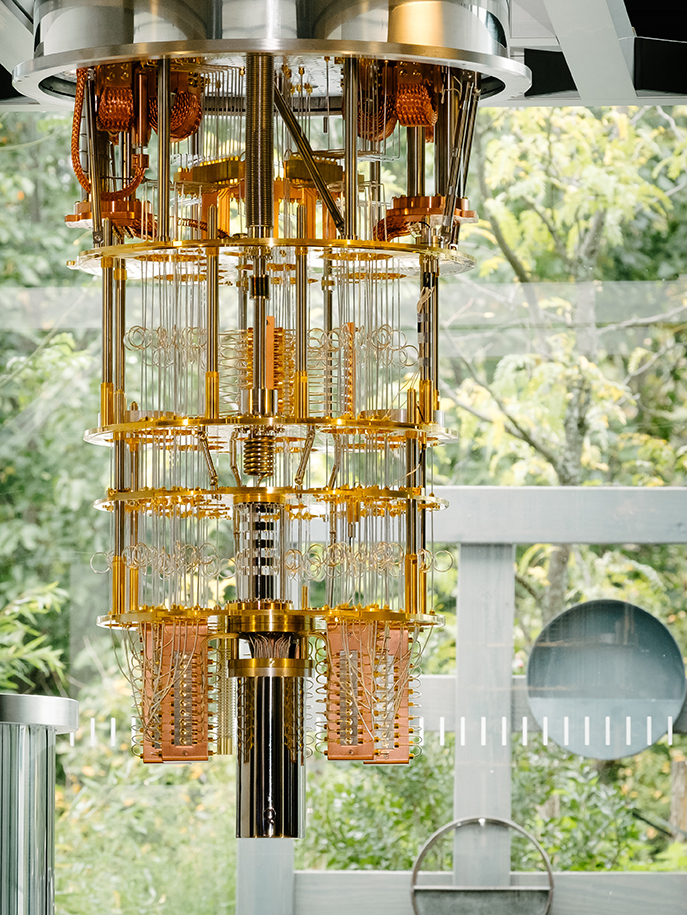
\includegraphics[width=0.75\linewidth]{Graphics/CEO-Forum_IBM-50Q-system_thumb.jpg}
      \caption{IBM Q dilution refrigerator (\SI{15}{\milli\kelvin}) and interface wiring to 50 superconducting charge qubits (transmons)~\cite{IBMQ-blog}}
    \end{figure}

    % Column 2
    \column[T]{0.33\linewidth}
    \begin{figure}
      \centering
      \caption{Xanadu cluster state photonic computer on chip (electronics
        and controls not shown)~\cite{Xanadu-Hardware}}
      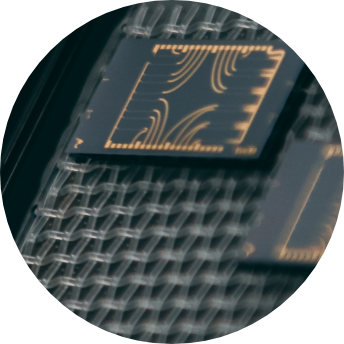
\includegraphics[width=0.48\linewidth]{Graphics/xanadu-chips-circle.png}    
      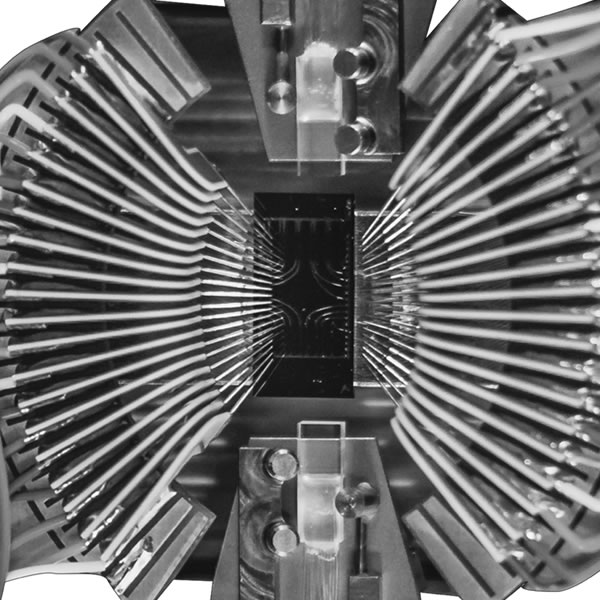
\includegraphics[width=0.48\linewidth]{Graphics/xanadu-control-systems.jpg}
    \end{figure}    % Column 3
    \column[T]{0.33\linewidth}
    \begin{figure}
      \centering
      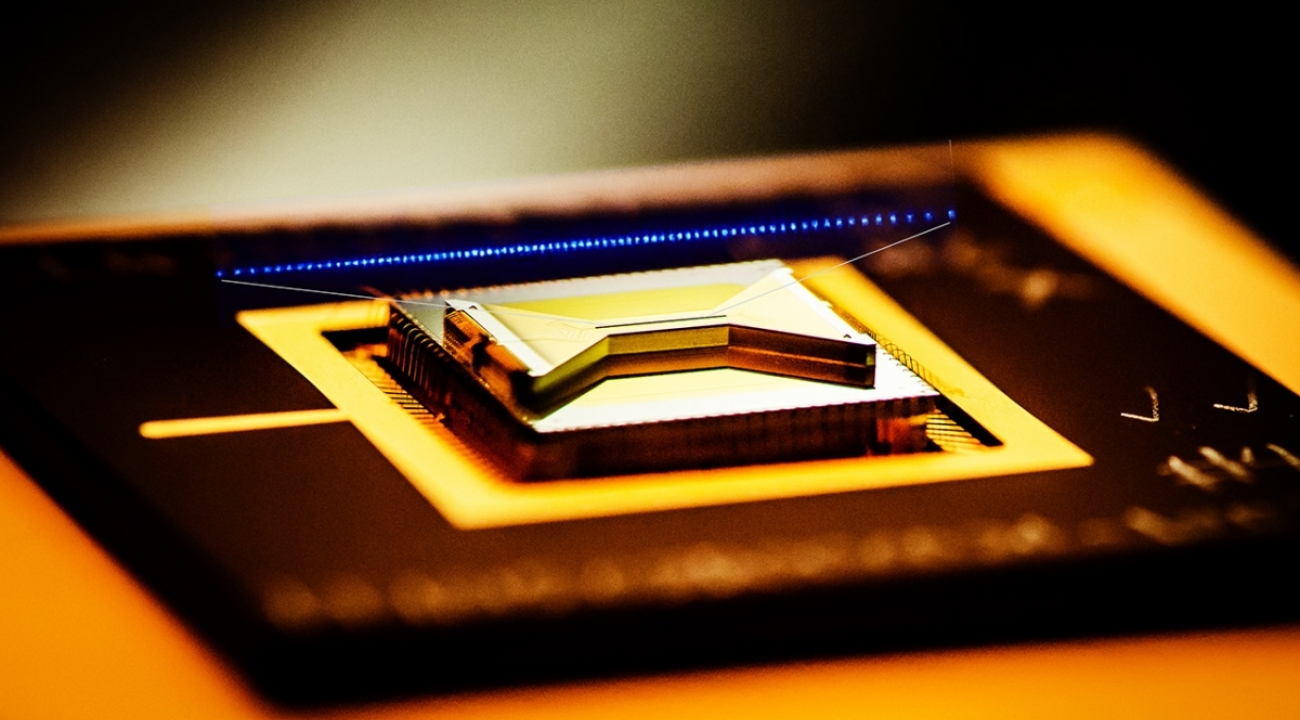
\includegraphics[width=0.95\linewidth]{Graphics/surface_trap-monroe-gallery.jpg}
      \caption{IonQ and Joint Quantum Institute atomic ion trap (laser
        cooling, atomic manipulation controls, and electronics not
        shown)~\cite{JQI-15M-NSF-news}}
    \end{figure}
  \end{columns}
\end{frame}
